\chapter{Background}
In this chapter we introduce fundamental theoretical concepts utilized in our project. We first explain the FSK modulation and demodulation. We then introduce Barker codes, which we use for synchronization in the project. Finally, we talk about Hamming codes which we use for error correction.

\section{FSK Modulation and Demodulation}
Modulation and demodulation are fundamental processes in digital communication. Modulation converts digital data into an analog signal suitable for transmission, while demodulation extracts the original digital data from the received analog signal. 
\\\\
Frequency Shift Keying (FSK) is a digital modulation scheme where data is encoded by varying the frequency of a carrier signal. In Binary Frequency Shift Keying (BFSK), the simplest form of FSK, binary 1 and 0 are represented by two distinct frequencies. This method allows digital data to be transmitted over analog channels such as radio waves or acoustic signals \cite{watson1980fsk}.
\\ 
The demodulation of an BFSK signal involves extracting the transmitted binary data from the received analog waveform. One of them is \textit{Fast Fourier Transformation (FFT)} \cite{duhamel1990fast} where the frequency spectrum is analyzed to identify the dominant frequency at a given time. FFT overall provides accurate results, however, it can be computationally intensive and use a significant amount of memory. In instances where resources or hardware power is limited, FFT might not be a great match. Another demodulation method is \textit{zero-crossing detection} \cite{wall2003simple}. In this approach we count how often the signal crosses the zero amplitude point to determine the frequency. zero-crossing detection is susceptible to noise. In instances where we have a very noisy environment, zero-crossing detection might not be ideal. If noise is not a problem, then it represents a resource-efficient and simple but working demodulation method.
\\ \\
While there are several other variations of FSK like \textit{Continuous Phase FSK} or \textit{Gaussian FSK} \cite{\cite{couch2013digital}} and demodulation option, we will not discuss them in further detail as we only experimented with BFSK as our modulation scheme.

\section{Barker Codes}
\textit{Barker codes} are binary sequences with excellent autocorrelation properties, they were first developed by H.R. Barker \cite{barker1953group}. This makes them ideal for synchronization, as they are easy to spot, even in a very noisy environment where other synchronization methods may struggle. We know of a limited amount of Barker codes \cite{Coxson2008}, all shown in Table~\ref{tab:barker_codes}.
\begin{table}[h]
    \label{tab:barker_codes}
    \centering
    \renewcommand{\arraystretch}{1.3}
    \begin{tabular}{|c|l|}
        \hline
        \textbf{Length} & \textbf{Barker Code} \\ 
        \hline
        2 & \textcolor{green!50!black}{+1} \textcolor{red}{-1} \quad or \quad \textcolor{green!50!black}{+1} \textcolor{green!50!black}{+1} \\ 
        \hline
        3 & \textcolor{green!50!black}{+1} \textcolor{green!50!black}{+1} \textcolor{red}{-1} \\ 
        \hline
        4 & \textcolor{green!50!black}{+1} \textcolor{red}{-1} \textcolor{green!50!black}{+1} \textcolor{green!50!black}{+1} \quad or \quad \textcolor{green!50!black}{+1} \textcolor{red}{-1} \textcolor{red}{-1} \textcolor{red}{-1} \\ 
        \hline
        5 & \textcolor{green!50!black}{+1} \textcolor{green!50!black}{+1} \textcolor{green!50!black}{+1} \textcolor{red}{-1} \textcolor{green!50!black}{+1} \\ 
        \hline
        7 & \textcolor{green!50!black}{+1} \textcolor{green!50!black}{+1} \textcolor{green!50!black}{+1} \textcolor{red}{-1} \textcolor{red}{-1} \textcolor{green!50!black}{+1} \textcolor{red}{-1} \\ 
        \hline
        11 & \textcolor{green!50!black}{+1} \textcolor{green!50!black}{+1} \textcolor{green!50!black}{+1} \textcolor{red}{-1} \textcolor{red}{-1} \textcolor{red}{-1} \textcolor{green!50!black}{+1} \textcolor{red}{-1} \textcolor{red}{-1} \textcolor{green!50!black}{+1} \textcolor{red}{-1} \\ 
        \hline
        13 & \textcolor{green!50!black}{+1} \textcolor{green!50!black}{+1} \textcolor{green!50!black}{+1} \textcolor{green!50!black}{+1} \textcolor{green!50!black}{+1} \textcolor{red}{-1} \textcolor{red}{-1} \textcolor{green!50!black}{+1} \textcolor{green!50!black}{+1} \textcolor{red}{-1} \textcolor{green!50!black}{+1} \textcolor{red}{-1} \textcolor{green!50!black}{+1} \\ 
        \hline
    \end{tabular}
    \caption{All Barker codes.}
    \label{tab:barker_codes}
\end{table}
The autocorrelation function of a Barker code exhibits minimal sidelobes, creating a strong peak when correlated with itself. This allows the receiver to detect its presence and clearly differentiate it from noise. Figure~\ref{fig:barker_code} illustrates the autocorrelation function of a 7-bit Barker code, the peak at zero shift is clearly visible.
\begin{figure}[h]
    \centering
    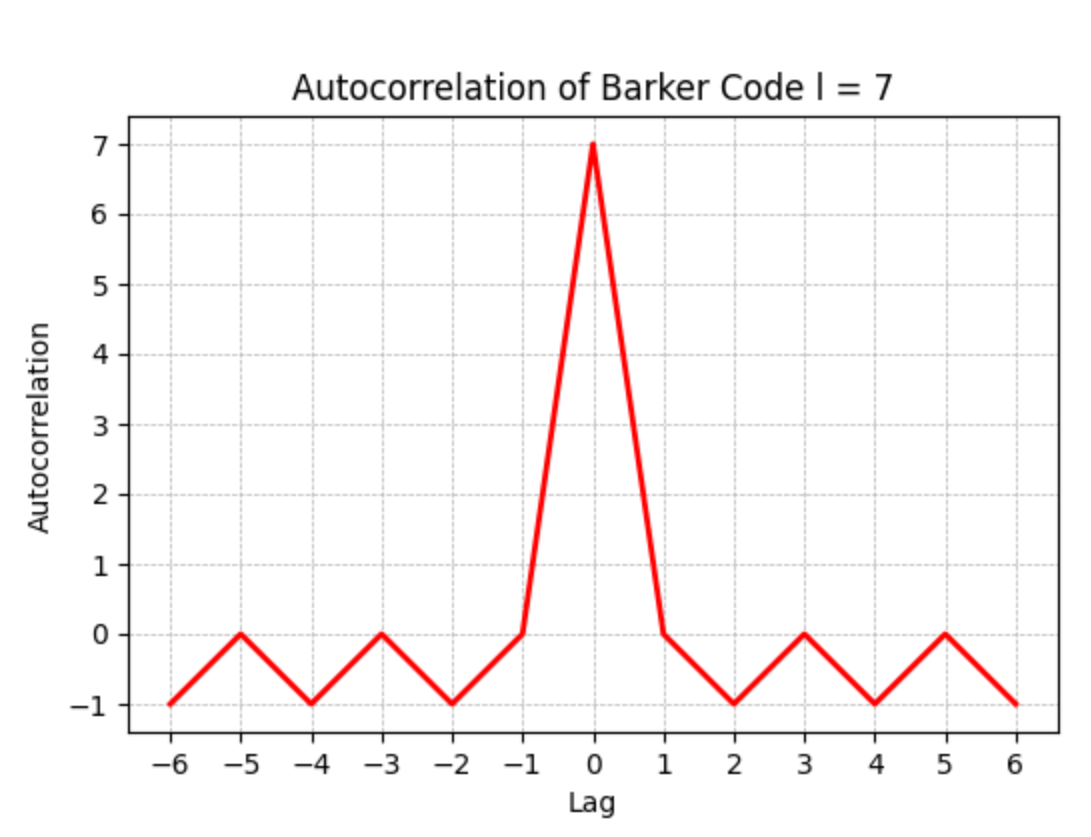
\includegraphics[scale=0.45]{images/ugly_barker_code.PNG}
    \caption{Autocorrelation function of the Barker code of length 7. The image was generated by the authors using Python.}
    \label{fig:barker_code}
\end{figure}
Despite their advantages, Barker codes have some limitations. The first is their limited length. There are no Barker codes longer than 13 bits, which limits their use to short synchronization sequences. Furthermore, Barker codes do not provide error correction, they only improve synchronization. In noisy conditions, additional steps must be taken.
\\ \\
Barker codes are used in various real-world applications such as radar systems, Code Division Multiple Access (CDMA) or GPS synchronization.

\section{Hamming Code}
\textit{Hamming codes} are a family of error-detecting and error-correcting codes developed by Richard Hamming \cite{hamming1950error}. They are used in digital communication to detect and correct single-bit errors. Transmission can obtain errors through noise, interference or signal degradation and lead to a misinterpretation of the data. Therefore, it is essential to detect and correct possible errors. Hamming codes achieve this by including parity bits to the data.
\\ \\
A Hamming code \textit{(n, k)} is an encoding scheme where we have a codeword of length $n$, $k$ data bits and $n-k$ redundant bits, also called parity bits. The parity bits are what enables Hamming codes to detect and correct errors. For example, a Hamming (7, 4) code contains 4 data bits and 3 parity bits. Via the XOR operator, the receiver can recalculate the parity bits and compare them with the received values. However, Hamming codes can only identify and correct a single corrupted bit. They can also detect two flipped bits, but not correct them. Error detection and correction of three or more errors is not possible, more robust error correction techniques would be needed. 
\\ \\
Including error correction of any kind introduces overhead, for example in Hamming codes parity bits are needed which reduce the transmission rate. Alternatives such as Reed-Solomon however cause even greater overhead, but are also more powerful in comparison. Hamming codes are however still efficient enough if we do not expect many errors in transmission, for example if we do not send information in noisy environments.